\section{噪声下限}\label{sec:noise}

现实噪声让谱相位掩模在 Mackey--Glass 上的误差从 $1.8\times10^{-6}$ 升到 $3.3\times10^{-4}$，差约 180 倍（表~\ref{tab:encodings}）。
第~\ref{sec:mechanism}~节说明，掩模工作在相干种子区，误差来自噪声而不是不可重复的动力学。
本节把五项噪声拆开，回答三个问题：下限由哪几项决定；换用非线性更强的材料、加功率能不能降低它；它能不能在读出端扣除。
结论是：下限约一半来自失谐抖动、一半来自散粒噪声；前一半与光子数无关；后一半虽然随光子数下降，但光子一多，前一半就成为主导，所以换 Si$_3$N$_4$ 和加功率都几乎无效；
把真实的抖动序列交给线性读出层只能去掉 2\% 的误差，所以抖动只能在光源处压低，这给出对激光线宽的要求。

\subsection{逐项拆分}\label{sec:breakdown}

为了把探测器的影响和器件内部的噪声分开，先假设探测器是理想的（没有电子噪声，只有散粒噪声），在 256 个随机工作点中按第~\ref{sec:protocol}~节的流程选出最优点，
再在这个点上一次只打开一项噪声（图~\ref{fig:noise}a）。
这个点的总功率为 $23~\mathrm{mW}$，总品质因数 $6\times10^{6}$，每根梳齿到达探测器约 $170~\mu\mathrm{W}$，即每个符号约 $1.3\times10^{6}$ 个光子。
它无噪声时的误差为 $1.3\times10^{-5}$。只打开激光强度噪声时为 $1.9\times10^{-5}$，几乎不变；
只打开腔内真空噪声时为 $2.5\times10^{-5}$；只打开失谐抖动时为 $5.7\times10^{-5}$；只打开散粒噪声时为 $6.8\times10^{-5}$。
三项光学噪声一起为 $7.8\times10^{-5}$，再加上散粒噪声为 $1.5\times10^{-4}$。
所以理想探测器下的误差下限约为 $1.3\times10^{-4}$（256 个点重新选点后的值），其中约一半来自失谐抖动，一半来自散粒噪声，
腔内真空噪声次要，激光强度噪声可以忽略。

换成现实的 PIN 探测器（每根梳齿 $0.3~\mu\mathrm{W}$ 的电子噪声），同样流程选出的最优点为 $3.4\times10^{-4}$，又差约 2.5 倍。
探测器噪声的影响在一个较早、较小规模的搜索（每种编码 32 个候选点，单次运行选点）中看得最清楚：
全部噪声打开、探测器噪声为 $0.03$、$0.1$、$0.3$、$0.6~\mu\mathrm{W}$ 时，误差为
$2.7\times10^{-4}$、$4.1\times10^{-4}$、$1.0\times10^{-3}$、$2.2\times10^{-3}$，在 $0.1~\mu\mathrm{W}$ 以上近似随探测器噪声线性增长；
在 $0.3~\mu\mathrm{W}$ 的探测器前加一级增益 $10~\mathrm{dB}$ 或 $20~\mathrm{dB}$、噪声系数 $5~\mathrm{dB}$ 的光放大器，误差降到 $3.3\times10^{-4}$ 和 $3.1\times10^{-4}$，
接近只有光学噪声和散粒噪声时的 $2.4\times10^{-4}$。
这个搜索的绝对数值与表~\ref{tab:encodings} 不能直接比（候选点少、选点方式不同），这里只用它看趋势：
探测器电子噪声是可以用光放大器去掉的一项，去掉之后剩下的就是上面的下限。

\begin{figure}[htbp]
\centering
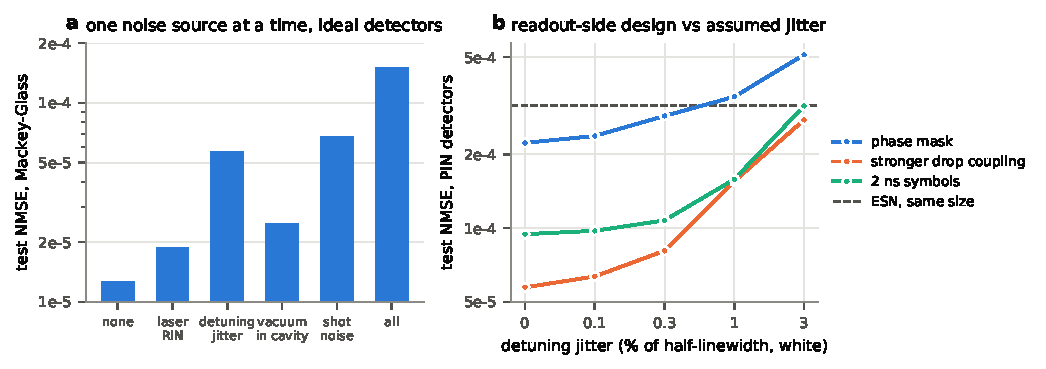
\includegraphics[width=\linewidth]{fig6_noise}
\caption{噪声与读出侧设计（Mackey--Glass）。
（a）理想探测器下，在 256 个点中选出的最优工作点上一次只打开一项噪声时的测试误差；“all”为四项（激光强度噪声、失谐抖动、腔内真空噪声、散粒噪声）同时打开；点线为同一点无噪声时的值。(a)(b) 中各点均为 3 条序列、每条 6 对新运行的几何平均。
（b）每档抖动重新选点后的测试误差随所假设的失谐抖动（每符号均方根，以半线宽的百分比计，相邻符号相关系数 $e^{-1}$；横轴为类别轴）的变化，PIN 探测器：
普通的谱相位掩模、加大下载端口耦合、$2~\mathrm{ns}$ 符号；虚线为同读出维度的 ESN（输入噪声 $3\times10^{-3}$，一个随机储备池）。
上方横轴是加大下载端口耦合工作点（$Q=1.9\times10^{6}$，$1~\mathrm{ns}$）上产生同样抖动的激光本征线宽（式~\eqref{eq:linewidth}）；$2~\mathrm{ns}$ 符号的工作点（$Q=5\times10^{6}$）约为其 0.3 倍。}
\label{fig:noise}
\end{figure}

\subsection{换非线性更强的材料、加功率都动不了下限}\label{sec:platform}

散粒噪声带来的误差可以靠更多光子来降低，失谐抖动则不能：抖动是相对于谐振线宽定义的，与腔内有多少光子无关。
我们用两种方式增加或减少光子数，并在每种情况下重新搜索 256 个工作点（理想探测器）：
\begin{itemize}
\item 换成 Si$_3$N$_4$ 微环（非线性系数约为石英的 60 倍，功率范围按 $\gamma L$ 的比例缩小，使归一化泵浦覆盖同样的范围）：
      最优点只需 $5~\mathrm{mW}$，到达探测器的光子少了约 8 倍，但误差下限为 $1.4\times10^{-4}$，与石英的 $1.3\times10^{-4}$ 相同；
\item 石英微环，功率范围提高到 10 倍（$0.1$ 到 $3~\mathrm{W}$）：误差下限为 $1.5\times10^{-4}$，没有改善。
      在它的最优点，每根梳齿的光子数是上面那个点的 4.4 倍，但散粒噪声那一项只从 $6.8\times10^{-5}$ 降到 $5.3\times10^{-5}$，
      失谐抖动那一项（$5.1\times10^{-5}$）则基本不变。
\end{itemize}
散粒噪声那一项的下降远慢于光子数的增加，但这两个最优点的其他参数也不同，所以这只是一个粗略的比较。
一个受控的比较是固定工作点和腔内动力学，只改变每个读数探测到的光子数（最好的单环，理想探测器，3 条序列 $\times$ 6 对新运行）：
光子数为原来的 1、10、100 倍时，总误差为 $1.41\times10^{-4}$、$1.21\times10^{-4}$、$1.16\times10^{-4}$，
没有散粒噪声时为 $1.16\times10^{-4}$。散粒噪声那一项本身随光子数下降（10 倍光子降约 5 倍，100 倍降约 40 倍），
但总误差很快停在光学噪声（主要是失谐抖动）决定的水平上。在这个工作点上，加功率最多只能把误差降低约 18\%。
换 Si$_3$N$_4$ 的好处在功率：同样的下限只需约 1/4 的功率；但在普通探测器下，到达探测器的光少了，误差反而升到 $1.1\times10^{-3}$，
要配更好的探测器或光放大器才能用上。
能降低下限的是读出一侧：加大下载端口耦合（让更多光到达探测器）或把符号放慢到 $2~\mathrm{ns}$（每个读数积分更久），
理想探测器下分别降到 $8.7\times10^{-5}$ 和 $6.9\times10^{-5}$，普通探测器下为 $1.55\times10^{-4}$ 和 $1.58\times10^{-4}$（第~\ref{sec:readout}~节）。

\subsection{知道真实抖动的线性读出层也没有去掉它}\label{sec:reference}

如果失谐抖动主要来自泵浦激光的频率噪声，那么同一芯片上、由同一台激光驱动的所有微环都看到同样的抖动。
一个自然的想法是加一个不加信号的参考环，测出这部分共模噪声，让读出层把它减掉。
我们先测这个想法的上限：在最好的单环（加大下载端口耦合组，$Q=1.9\times10^{6}$，$178~\mathrm{mW}$）上，
直接把每次运行真实的抖动序列（当前和前 7 个符号）交给读出层，相当于一个没有噪声的理想参考。
3 条序列、每条 6 对新运行的结果是：原样读出为 $1.60\times10^{-4}$；加上真实抖动序列后为 $1.58\times10^{-4}$，只降 2\%；
再加上当前抖动与各梳齿特征的乘积项（让修正量可以随状态变化），反而略差，为 $1.65\times10^{-4}$。
而把抖动本身关掉、其余噪声不变时，误差降到 $5.7\times10^{-5}$，好 2.8 倍。

也就是说，抖动确实是下限的大头，但即使完全知道它，我们试过的线性读出也只去掉 2\% 的误差。
可能的原因是抖动不是叠加在读数上的加性噪声：它改变了腔内的失谐，经过非线性动力学改变了整个梳的状态，而且这个影响会延续到后面几个符号；
它对每根梳齿的作用取决于当时的状态，线性读出层去不掉它。
所以用线性读出的共参考环不成立。我们没有把参考环自己的 31 路梳齿特征（它们是抖动历史的非线性函数）交给读出层。
对梳齿特征取二次项的读出层（第~\ref{sec:nonlin-readout}~节）对有、无抖动的误差同样降低，抖动损失仍为 2.7；最直接的办法还是在物理上压低抖动。

\subsection{没有找到对抖动不敏感的工作点}\label{sec:sweetspot}

在谐振峰顶，透射功率对失谐是驻点，抖动只能以二阶形式进来。Kerr 频移和色散使这一点不可能对每个输入、每根梳齿同时成立，但也许存在一片敏感性较低的区域。
我们在最好的单环周围扫了 78 个点（归一化失谐 $-1$ 到 $4$、步长 $0.2$；功率为原来的 0.5、1、1.5 倍），每个点在 3 条序列上各用 3 对新运行，分别测有、无抖动的误差。
抖动损失接近 1 的点确实存在，但那里无抖动时的误差就有 $3\times10^{-3}$ 到 $2\times10^{-2}$；无抖动误差低于 $2\times10^{-4}$ 的 10 个点，抖动损失都在 1.4 到 3.5 之间，
在全部点上两者呈负相关（对数的相关系数为 $-0.66$）。有抖动时最好的点为 $1.28\times10^{-4}$，不比原工作点好。

可能的原因是信号和抖动走同一条通道。掩模调制腔内功率，主要通过 Kerr 频移改变有效失谐来作用于整个梳；抖动改变的也是这个失谐。
微环在某点算得好，正是因为它在那里对失谐响应强，因而对抖动也敏感。这与线性和二次读出都分不开两者的结果一致，
也促使我们把信号送进另一组共享抖动、但信号符号相反的模式（第~\ref{sec:bidir}~节）。

\subsection{激光本征线宽的要求}\label{sec:laser}

上面的噪声模型给每个符号一个均方根为半线宽 1\% 的失谐抖动。现在把它和激光联系起来。
设激光的频率噪声是白噪声，对应洛伦兹线宽 $\Delta\nu$（单边频率噪声谱 $S_\nu=\Delta\nu/\pi$），
则在一个符号时间 $T$ 内平均后的频率起伏方差为 $\Delta\nu/(2\pi T)$。
以谐振的半线宽 $\nu_0/(2Q)$ 为单位，每个符号的相对抖动 $\varepsilon$ 与线宽的关系为
\begin{equation}
\Delta\nu=2\pi T\left(\frac{\varepsilon\,\nu_0}{2Q}\right)^{2}.
\label{eq:linewidth}
\end{equation}
对最好的单环（$Q=1.9\times10^{6}$，半线宽 $51~\mathrm{MHz}$，$T=1~\mathrm{ns}$），1\% 的抖动对应约 $1.6~\mathrm{kHz}$ 的本征线宽，
0.3\% 和 0.1\% 分别对应约 $150~\mathrm{Hz}$ 和 $16~\mathrm{Hz}$；反过来，本征线宽 $100~\mathrm{kHz}$ 的激光会带来约 8\% 的抖动。
所需线宽随 $Q$ 的平方变严，随符号时间变松：第~\ref{sec:readout}~节 $2~\mathrm{ns}$ 符号的工作点 $Q=5\times10^{6}$，1\% 对应约 $470~\mathrm{Hz}$。

为了检验这个换算，我们直接按真实激光的频率噪声谱生成抖动：$S_\nu(f)=h_0+h_{-1}/f$，
其中 $h_0=\Delta\nu/\pi$ 是白频率噪声，$h_{-1}/f$ 是闪烁噪声（半导体激光的转折频率通常在 $1~\mathrm{MHz}$ 左右）；
激光被锁在谐振上，锁定环路对频率噪声的抑制用一个一阶高通 $f^{2}/(f^{2}+B^{2})$ 表示。
时间序列由频谱合成，在每个符号内平均，再除以半线宽，作为每次运行的失谐抖动；其余噪声不变。
表~\ref{tab:laser} 给出结果。

% generated by experiments/make_table2.py; do not edit by hand
\begin{table}[htbp]
\centering
\caption{真实激光下最好的单环（加大下载端口耦合组，Mackey--Glass，现实噪声的其余各项不变）。失谐抖动由激光的白频率噪声按每个符号平均得到；“固定工作点”是 1\% 抖动假设下选出的点（$Q=1.9\times10^{6}$），“重选”是在该激光的噪声下按第~\ref{sec:protocol}~节的流程重新选点（每条序列 56 个按 $Q$ 分档的候选）。3 条序列 $\times$ 6 对新运行。两列用了不同的噪声实现，同一个工作点在两列之间约有 9\% 的差别。}
\label{tab:laser}
\small
\begin{tabular}{p{4.2cm}cccc}
\toprule
激光本征线宽 & 每符号抖动 & 固定工作点 & 重选后 & 重选点的 $Q$ \\
\midrule
100~Hz & 0.25\% & $6.7\times10^{-5}$ & -- & -- \\
1.6~kHz & 1.00\% & $1.3\times10^{-4}$ & $1.2\times10^{-4}$ & $1.9\times10^{6}$ \\
16~kHz & 3.15\% & $3.1\times10^{-4}$ & $2.9\times10^{-4}$ & $1.9\times10^{6}$ \\
100~kHz & 7.88\% & $8.1\times10^{-4}$ & $6.4\times10^{-4}$ & $1.9\times10^{6}$、$2.5\times10^{6}$ \\
1~MHz & 24.92\% & $5.2\times10^{-3}$ & $1.6\times10^{-3}$ & $1.2\times10^{6}$ \\
\midrule
100~kHz，加闪烁噪声（转折 1~MHz）和 1~MHz 锁定 & 7.92\% & $8.3\times10^{-4}$ & -- & -- \\
1.6~kHz，加闪烁噪声（转折 10~MHz），不锁定 & 1.10\% & $1.8\times10^{-4}$ & -- & -- \\
\bottomrule
\end{tabular}
\end{table}


表~\ref{tab:laser} 给出四点。
第一，在纳秒符号下起决定作用的是本征（白噪声）线宽：一个 $1~\mathrm{ns}$ 符号对应约 $500~\mathrm{MHz}$ 的带宽，几乎全被白频率噪声占据，
而闪烁噪声的功率集中在低频；加入转折频率 $1~\mathrm{MHz}$ 的闪烁噪声和 $1~\mathrm{MHz}$ 的锁定后，$100~\mathrm{kHz}$ 那一行几乎不变；
只有闪烁噪声极强（转折 $10~\mathrm{MHz}$）且完全不锁定时，$1.6~\mathrm{kHz}$ 那一行才从 $1.3\times10^{-4}$ 变为 $1.8\times10^{-4}$。
第二，本文的 1\% 抖动模型（相邻符号相关系数 $e^{-1}$）在这个点上给出 $1.60\times10^{-4}$，比同样均方根的白频率噪声（$1.27\times10^{-4}$）偏悲观约 25\%，
所以在这个点上前面的主要结果略偏保守（这个点用其他噪声实现评估时为 $1.5$ 到 $1.6\times10^{-4}$，我们取第~\ref{sec:readout}~节的 $1.55\times10^{-4}$ 作为参考值）。
第三，换工作点绕不开这个要求：在 $1.6~\mathrm{kHz}$ 和 $16~\mathrm{kHz}$ 下重新选点仍选回原来的点；
$100~\mathrm{kHz}$ 时有两条序列换成 $Q=2.5\times10^{6}$ 的点，误差改善约 1.3 倍，比同一工作点在不同噪声实现之间约 9\% 的差别大，但幅度有限；
只有 $1~\mathrm{MHz}$ 时选点明显移向较低的 $Q$（$1.2\times10^{6}$），误差改善 3.3 倍，但候选中最低的 $Q$（约 $5\times10^{5}$）从未被选中，
因为低 $Q$ 的点非线性和记忆都弱，抖动减小的好处被抵消了。
第四，与软件的位置：输入噪声 $3\times10^{-3}$ 的 31 节点 ESN 为 $1.9\times10^{-4}$（3 个储备池）到 $3.2\times10^{-4}$（1 个储备池）；
按表~\ref{tab:laser} 对数插值，本征线宽需在约 $5$ 到 $17~\mathrm{kHz}$ 以下，最好的单环才不输于它。以 $1.9\times10^{-4}$ 为准，$100~\mathrm{kHz}$ 的激光使微环比 ESN 差约 4 倍，$1~\mathrm{MHz}$ 的激光即使重选工作点也差约 8 倍。

这给出第二条设计规则：\emph{误差下限的一半由激光相对谐振的频率噪声决定，知道真实抖动的线性读出层没有去掉它，重新选工作点也没有绕开它，需要窄线宽的光源}。
对本文的器件（$Q\sim2\times10^{6}$、$1~\mathrm{GBd}$），激光本征线宽应在几千赫兹以下。
把激光自注入锁定到微环上，是已知的把半导体激光线宽压窄几个数量级的办法~\cite{shen2020,jin2021}：
例如把普通分布反馈（DFB）激光自注入锁定到 $Q>2.6\times10^{8}$ 的氮化硅微环上，频率噪声降低约五个数量级，短时线宽达到约 $1.2~\mathrm{Hz}$~\cite{jin2021}，
比本文要求的几千赫兹低得多。
环自身的热折射噪声没有计入，它主要在低频，在锁定之后对纳秒尺度的影响预计较小，但需要单独核实。
